% =========================================================================== %
% Yes. This is a document.

\documentclass[
	ngerman,
	aspectratio=169,
	table
]{beamer}

% =========================================================================== %
% Theme
\usepackage{scrlfile}
	\ReplacePackage{beamerthemeSHUR}{./sty/beamerthemeSHUR}
	\ReplacePackage{beamerinnerthemefancy}{./sty/beamerinnerthemefancy}
	\ReplacePackage{beamerouterthemedecolines}{./sty/beamerouterthemedecolines}
	\ReplacePackage{beamercolorthemechameleon}{./sty/beamercolorthemechameleon}

\usetheme[
	pageofpages=von,
	bullet=circle,
	titleline=true,
	alternativetitlepage=true,
	watermark="",
	watermarkheight=0px,
	watermarkheightmult=0
	]
{SHUR}

% =================================================================================================== %
% the usual stuff

\usepackage[utf8]{inputenc}
\usepackage[T1]{fontenc}
\usepackage{babel}
\usepackage{lmodern}
\usepackage{microtype}
\usepackage{csquotes}

\usepackage{tabularx}
\usepackage{booktabs}
\usepackage{multirow}

\usepackage{color, colortbl}
\usepackage{xcolor}

\usepackage{tabto}

\usepackage{minted}
	\usemintedstyle{friendly}

\usepackage{tikz}
	\usetikzlibrary{positioning}
	\usetikzlibrary{matrix}
	\usetikzlibrary{shapes.geometric}
	\usetikzlibrary{backgrounds}
	\usetikzlibrary{calc}
	\usetikzlibrary{decorations.pathreplacing}
	\tikzstyle{every picture}+=[remember picture] 
\usepackage{adjustbox}

\usepackage[most]{tcolorbox}
	\tcbsetforeverylayer
		{colback=cyan!10!white,
		 colframe=cyan!75!black,
		 arc=0pt,
		 outer arc=0pt
		}
	\newtcolorbox{codebox}[1][Code]
		{colback=black!5!white,
		 colframe=blue!40!black,
		 title=#1,
		 leftupper=6mm
		}
	\newtcolorbox{cmdbox}[1][Kommandozeilen-Befehl]
		{colback=black,
		 coltext=white,
		 fontupper=\ttfamily ,
		 colframe=blue!40!black,
		 title=#1,
		 outer arc=0pt
		}
	\newtcolorbox{warnbox}[1][Beachte]
		{colback=black!5!white,
		 colframe=red!40!black,
		 title=#1
		}
	\newtcolorbox{hintbox}[1][Tipp]
		{colback=black!5!white,
		 colframe=green!40!black,
		 title=#1
		}%
	\newenvironment{itembox}[1][]
		{\begin{tcolorbox}[title=#1]\begin{itemize}}%
		{\end{itemize}\end{tcolorbox}}
	\newtcolorbox{doublebox}[1][.3]
		{righthand width=#1\linewidth,
		 sidebyside,
		 sidebyside gap=6mm,
		 sidebyside align=center,
		 lower separated=false}

%==============================================================================%
% GLOBAL MACROS

\newcommand*{\zB}{z.\,B. }
\newcommand*{\ua}{u.\,a. }
\newcommand*{\ie}{d.\,h. }			%% dh is already a defined macro. Couldn't find out what it does.
\newcommand*{\idR}{i.\,d.\,R. }

\newcommand*{\tabcrlf}{\\ \midrule}			% actually still allows for optional argument

% =========================================================================== %

\author{Stefan Hartinger}
\title{Programmieren in C und C++}
\subtitle{Kursteil 15: Linked Lists}
\institute{Universität Regensburg, Fakultät Physik}
\date{Wintersemester 2019/20}

% =========================================================================== %

\begin{document}
% =========================================================================== %

\begin{frame}[t,plain]
\titlepage
\end{frame}

% =========================================================================== %

\begin{frame}[fragile]{Recap}
%
\begin{itemize}
\item Datei-Management
	\begin{itemize}
	\item Zugriff über \emph{handles}:\tabto{4cm} \texttt{FILE * fp = fopen("filename", "mode");}
	\item Modi: Lesen (\texttt{r}), Schreiben (\texttt{w}), Anhängen (\texttt{a})
	\item Schreiben mit \texttt{fprintf} oder \texttt{fwrite}
	\item Lesen mit \texttt{fscanf} oder \texttt{fread}
	\item Schließen/Datei freigeben mit \texttt{fclose}
	\end{itemize}
\item Rekursion
	\begin{itemize}
	\item Funktionen, die sich selbst aufrufen
	\item Zerlegung in einfachere Unterprobleme
	\item Eigener Scope für jede Instanz
	\end{itemize}
\item Fragen?
\end{itemize}
%
\end{frame}

% =========================================================================== %

\begin{frame}{Script}

\begin{itemize}
\item Kapitel 17
	\begin{itemize}
	\item 17.1. Ausgangslage: Klassische Arrays
	\item 17.2. Verknüpfung mit seinen Nachbarn: Linked Lists
	\item 17.3. Aufbau einer Bibliothek zur Verwaltung von Linked Lists
	\item 17.4. Einsatzbereiche der Linked List: Vor- und Nachteile 
	\end{itemize}
\end{itemize}

\end{frame}

% =========================================================================== %

\begin{frame}[fragile]
%
\begin{columns}[T]
\column{.4\linewidth}
\begin{Large}
Linked List: Ausgangsproblem
\vspace{10pt}
\end{Large}
%
\begin{itemize}
\item Aufgabe: Füge Element in Liste ein
\item Nötige Schritte:
	\begin{itemize}
	\item Mehr Speicherplatz allozieren
	\item Elemente \enquote{um einen Platz verschieben}
	\item Neues Element schreiben
	\end{itemize}
\item Bei häufigem Einfügen oder großen Datenmengen: Langsam
\end{itemize}
%
\column{.6\linewidth}
\begin{codebox}[Beispiel: Wert Einfügen]
\begin{minted}[fontsize=\scriptsize, linenos]{c}
int * insert(
   int * lst, int len, int pos, int new
) {
   lst = realloc(
      lst, 
      (len + 1) * sizeof(int)
   );
   if (!lst) {
      printf("failure.\n"); 
      return NULL;
   }
   
   for (int i = len; i > pos; i--) {
      lst[i] = lst[i-1];
   }
   
   lst[pos] = new;
   return lst;
}
\end{minted}
\end{codebox}
\end{columns}

%
\end{frame}

% =========================================================================== %

\begin{frame}[fragile]
%
\begin{codebox}[Datentyp für Elemente einer Linked List]
\begin{minted}[linenos, fontsize=\scriptsize]{c}
typedef struct listElement_struct {
  int                         data;
  struct listElement_struct * next;
} listElement_t;
\end{minted}
\end{codebox}
%
\begin{tcolorbox}[title=Visualisierung: Verkettete Liste]
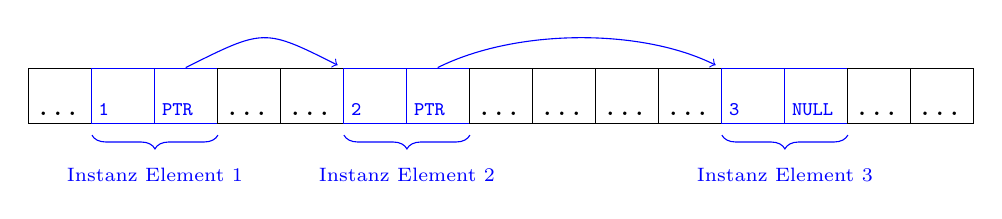
\begin{tikzpicture}
  [ 
    cell/.style={text width=6mm,
    text height=5mm, draw=black, inner sep=1mm},
    ld/.style={draw=blue,shorten >=2pt,->}
  ]
  \node (c01) at ( 0.0,0) [cell]       {\ttfamily \ldots};
  \node (c02) at ( 0.8,0) [cell, blue] {\ttfamily \scriptsize 1};
  \node (c03) at ( 1.6,0) [cell, blue] {\ttfamily \scriptsize PTR};
  \node (c04) at ( 2.4,0) [cell]       {\ttfamily \ldots};
  \node (c05) at ( 3.2,0) [cell]       {\ttfamily \ldots};
  \node (c06) at ( 4.0,0) [cell, blue] {\ttfamily \scriptsize 2};
  \node (c07) at ( 4.8,0) [cell, blue] {\ttfamily \scriptsize PTR};
  \node (c08) at ( 5.6,0) [cell]       {\ttfamily \ldots};
  \node (c09) at ( 6.4,0) [cell]       {\ttfamily \ldots};
  \node (c10) at ( 7.2,0) [cell]       {\ttfamily \ldots};
  \node (c11) at ( 8.0,0) [cell]       {\ttfamily \ldots};
  \node (c12) at ( 8.8,0) [cell, blue] {\ttfamily \scriptsize 3};
  \node (c13) at ( 9.6,0) [cell, blue] {\ttfamily \scriptsize NULL};
  \node (c14) at (10.4,0) [cell]       {\ttfamily \ldots};
  \node (c15) at (11.2,0) [cell]       {\ttfamily \ldots};
  
  \draw [ld] (c03.north) .. controls +(1.0,0.5) and +(-1.0, 0.5) .. (c06.north west);
  \draw [ld] (c07.north) .. controls +(1.0,0.5) and +(-1.0, 0.5) .. (c12.north west);
  
  \draw [decorate, decoration={brace, amplitude=5pt, mirror}, xshift=-4pt, yshift=0pt, blue]
  		(0.55, -0.5) -- (2.15, -0.5) 
  		node [midway, yshift=-0.5cm]
		(I1) {\scriptsize Instanz Element 1};
  \draw [decorate, decoration={brace, amplitude=5pt, mirror}, xshift=-4pt, yshift=0pt, blue]
  		(3.75, -0.5) -- (5.35, -0.5) 
  		node [midway, yshift=-0.5cm]
		(I2) {\scriptsize Instanz Element 2};
  \draw [decorate, decoration={brace, amplitude=5pt, mirror}, xshift=-4pt, yshift=0pt, blue]
  		(8.55, -0.5) -- (10.15, -0.5) 
  		node [midway, yshift=-0.5cm]
		(I3) {\scriptsize Instanz Element 3};
\end{tikzpicture}
\end{tcolorbox}
%
\end{frame}

% =========================================================================== %

\begin{frame}[fragile]
%
\begin{tcolorbox}[title=Visualisierung: Einfügen in eine verkettete Liste]
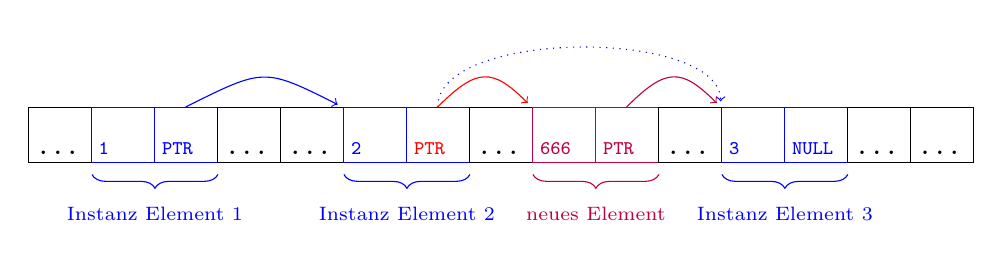
\begin{tikzpicture}
  [ 
    cell/.style={text width=6mm,
    text height=5mm, draw=black, inner sep=1mm},
    ld/.style={draw=blue,shorten >=2pt,->}
  ]
  \node (c01) at ( 0.0,0) [cell]         {\ttfamily \ldots};
  \node (c02) at ( 0.8,0) [cell, blue]   {\ttfamily \scriptsize 1};
  \node (c03) at ( 1.6,0) [cell, blue]   {\ttfamily \scriptsize PTR};
  \node (c04) at ( 2.4,0) [cell]         {\ttfamily \ldots};
  \node (c05) at ( 3.2,0) [cell]         {\ttfamily \ldots};
  \node (c06) at ( 4.0,0) [cell, blue]   {\ttfamily \scriptsize 2};
  \node (c07) at ( 4.8,0) [cell, blue]   {\ttfamily \scriptsize \textcolor{red}{PTR}};
  \node (c08) at ( 5.6,0) [cell]         {\ttfamily \ldots};
  \node (c09) at ( 6.4,0) [cell, purple] {\ttfamily \scriptsize 666};
  \node (c10) at ( 7.2,0) [cell, purple] {\ttfamily \scriptsize PTR};
  \node (c11) at ( 8.0,0) [cell]         {\ttfamily \ldots};
  \node (c12) at ( 8.8,0) [cell, blue]   {\ttfamily \scriptsize 3};
  \node (c13) at ( 9.6,0) [cell, blue]   {\ttfamily \scriptsize NULL};
  \node (c14) at (10.4,0) [cell]         {\ttfamily \ldots};
  \node (c15) at (11.2,0) [cell]         {\ttfamily \ldots};
  
  \draw [ld]         (c03.north) .. controls +(1.0,0.5) and +(-1.0, 0.5) .. (c06.north west);
  \draw [ld, dotted] (c07.north) .. controls +(0.0,1.0) and +(-0.0, 1.0) .. (c12.north west);
  \draw [ld, red]    (c07.north) .. controls +(0.5,0.5) and +(-0.5, 0.5) .. (c09.north west);
  \draw [ld, purple] (c10.north) .. controls +(0.5,0.5) and +(-0.5, 0.5) .. (c12.north west);

  \draw [decorate, decoration={brace, amplitude=5pt, mirror}, xshift=-4pt, yshift=0pt, blue]
  		(0.55, -0.5) -- (2.15, -0.5) 
  		node [midway, yshift=-0.5cm]
		(I1) {\scriptsize Instanz Element 1};
  \draw [decorate, decoration={brace, amplitude=5pt, mirror}, xshift=-4pt, yshift=0pt, blue]
  		(3.75, -0.5) -- (5.35, -0.5) 
  		node [midway, yshift=-0.5cm]
		(I2) {\scriptsize Instanz Element 2};
  \draw [decorate, decoration={brace, amplitude=5pt, mirror}, xshift=-4pt, yshift=0pt, blue]
  		(8.55, -0.5) -- (10.15, -0.5) 
  		node [midway, yshift=-0.5cm]
		(I3) {\scriptsize Instanz Element 3};
  \draw [decorate, decoration={brace, amplitude=5pt, mirror}, xshift=-4pt, yshift=0pt, purple]
  		(6.15, -0.5) -- (7.75, -0.5) 
  		node [midway, yshift=-0.5cm]
		(I4) {\scriptsize neues Element};
\end{tikzpicture}
%
\begin{itemize}
\item Neues Element vorbereiten
\item Zeigt auf Nachfolger
\item Pointer des Vorgängers updaten
\end{itemize}
\end{tcolorbox}
%
\end{frame}

% =========================================================================== %

\begin{frame}[fragile]
%
\begin{tcolorbox}[title=Visualisierung: Einfügen an das Ende einer verkettete Liste]
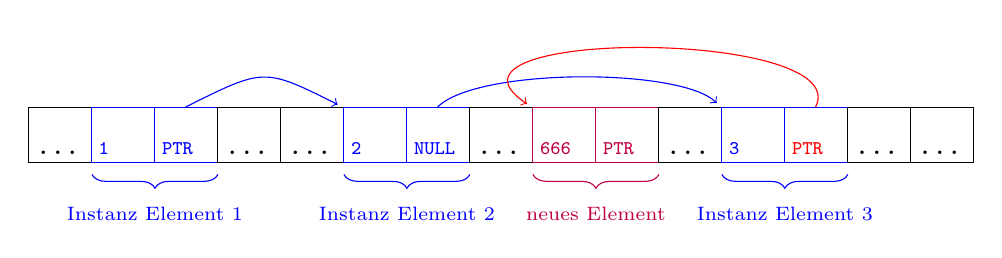
\begin{tikzpicture}
  [ 
    cell/.style={text width=6mm,
    text height=5mm, draw=black, inner sep=1mm},
    ld/.style={draw=blue,shorten >=2pt,->}
  ]
  \node (c01) at ( 0.0,0) [cell]         {\ttfamily \ldots};
  \node (c02) at ( 0.8,0) [cell, blue]   {\ttfamily \scriptsize 1};
  \node (c03) at ( 1.6,0) [cell, blue]   {\ttfamily \scriptsize PTR};
  \node (c04) at ( 2.4,0) [cell]         {\ttfamily \ldots};
  \node (c05) at ( 3.2,0) [cell]         {\ttfamily \ldots};
  \node (c06) at ( 4.0,0) [cell, blue]   {\ttfamily \scriptsize 2};
  \node (c07) at ( 4.8,0) [cell, blue]   {\ttfamily \scriptsize NULL};
  \node (c08) at ( 5.6,0) [cell]         {\ttfamily \ldots};
  \node (c09) at ( 6.4,0) [cell, purple] {\ttfamily \scriptsize 666};
  \node (c10) at ( 7.2,0) [cell, purple] {\ttfamily \scriptsize PTR};
  \node (c11) at ( 8.0,0) [cell]         {\ttfamily \ldots};
  \node (c12) at ( 8.8,0) [cell, blue]   {\ttfamily \scriptsize 3};
  \node (c13) at ( 9.6,0) [cell, blue]   {\ttfamily \scriptsize \textcolor{red}{PTR}};
  \node (c14) at (10.4,0) [cell]         {\ttfamily \ldots};
  \node (c15) at (11.2,0) [cell]         {\ttfamily \ldots};
  
  \draw [ld]         (c03.north) .. controls +(1.0,0.5) and +(-1.0, 0.5) .. (c06.north west);
  \draw [ld]         (c07.north) .. controls +(0.5,0.5) and +(-0.5, 0.5) .. (c12.north west);
  \draw [ld, red]    (c13.north) .. controls +(0.5,1.0) and +(-1.5, 1.0) .. (c09.north west);

  \draw [decorate, decoration={brace, amplitude=5pt, mirror}, xshift=-4pt, yshift=0pt, blue]
  		(0.55, -0.5) -- (2.15, -0.5) 
  		node [midway, yshift=-0.5cm]
		(I1) {\scriptsize Instanz Element 1};
  \draw [decorate, decoration={brace, amplitude=5pt, mirror}, xshift=-4pt, yshift=0pt, blue]
  		(3.75, -0.5) -- (5.35, -0.5) 
  		node [midway, yshift=-0.5cm]
		(I2) {\scriptsize Instanz Element 2};
  \draw [decorate, decoration={brace, amplitude=5pt, mirror}, xshift=-4pt, yshift=0pt, blue]
  		(8.55, -0.5) -- (10.15, -0.5) 
  		node [midway, yshift=-0.5cm]
		(I3) {\scriptsize Instanz Element 3};
  \draw [decorate, decoration={brace, amplitude=5pt, mirror}, xshift=-4pt, yshift=0pt, purple]
  		(6.15, -0.5) -- (7.75, -0.5) 
  		node [midway, yshift=-0.5cm]
		(I4) {\scriptsize neues Element};
\end{tikzpicture}
%
\begin{itemize}
\item Neues Element vorbereiten
\item Zeigt auf \texttt{NULL}
\item Pointer des vormals letzten Elements updaten
\end{itemize}
\end{tcolorbox}
%
\end{frame}

% =========================================================================== %

\begin{frame}
%
\begin{tcolorbox}[title=Visualisierung: Einfügen an den Anfang einer verkettete Liste]
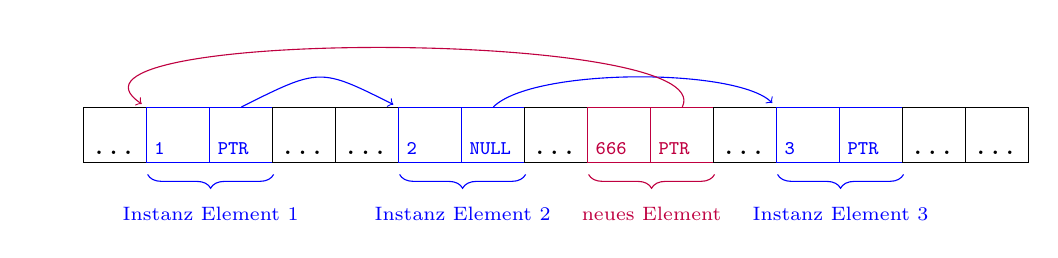
\begin{tikzpicture}
  [ 
    cell/.style={text width=6mm,
    text height=5mm, draw=black, inner sep=1mm},
    ld/.style={draw=blue,shorten >=2pt,->}
  ]
  \node (c01) at ( 0.0,0) [cell]         {\ttfamily \ldots};
  \node (c02) at ( 0.8,0) [cell, blue]   {\ttfamily \scriptsize 1};
  \node (c03) at ( 1.6,0) [cell, blue]   {\ttfamily \scriptsize PTR};
  \node (c04) at ( 2.4,0) [cell]         {\ttfamily \ldots};
  \node (c05) at ( 3.2,0) [cell]         {\ttfamily \ldots};
  \node (c06) at ( 4.0,0) [cell, blue]   {\ttfamily \scriptsize 2};
  \node (c07) at ( 4.8,0) [cell, blue]   {\ttfamily \scriptsize NULL};
  \node (c08) at ( 5.6,0) [cell]         {\ttfamily \ldots};
  \node (c09) at ( 6.4,0) [cell, purple] {\ttfamily \scriptsize 666};
  \node (c10) at ( 7.2,0) [cell, purple] {\ttfamily \scriptsize PTR};
  \node (c11) at ( 8.0,0) [cell]         {\ttfamily \ldots};
  \node (c12) at ( 8.8,0) [cell, blue]   {\ttfamily \scriptsize 3};
  \node (c13) at ( 9.6,0) [cell, blue]   {\ttfamily \scriptsize PTR};
  \node (c14) at (10.4,0) [cell]         {\ttfamily \ldots};
  \node (c15) at (11.2,0) [cell]         {\ttfamily \ldots};
  
  \draw [ld]         (c03.north) .. controls +(1.0,0.5) and +(-1.0, 0.5) .. (c06.north west);
  \draw [ld]         (c07.north) .. controls +(0.5,0.5) and +(-0.5, 0.5) .. (c12.north west);
  \draw [ld, purple] (c10.north) .. controls +(0.5,1.0) and +(-1.5, 1.0) .. (c02.north west);

  \draw [decorate, decoration={brace, amplitude=5pt, mirror}, xshift=-4pt, yshift=0pt, blue]
  		(0.55, -0.5) -- (2.15, -0.5) 
  		node [midway, yshift=-0.5cm]
		(I1) {\scriptsize Instanz Element 1};
  \draw [decorate, decoration={brace, amplitude=5pt, mirror}, xshift=-4pt, yshift=0pt, blue]
  		(3.75, -0.5) -- (5.35, -0.5) 
  		node [midway, yshift=-0.5cm]
		(I2) {\scriptsize Instanz Element 2};
  \draw [decorate, decoration={brace, amplitude=5pt, mirror}, xshift=-4pt, yshift=0pt, blue]
  		(8.55, -0.5) -- (10.15, -0.5) 
  		node [midway, yshift=-0.5cm]
		(I3) {\scriptsize Instanz Element 3};
  \draw [decorate, decoration={brace, amplitude=5pt, mirror}, xshift=-4pt, yshift=0pt, purple]
  		(6.15, -0.5) -- (7.75, -0.5) 
  		node [midway, yshift=-0.5cm]
		(I4) {\scriptsize neues Element};
\end{tikzpicture}
%
\begin{itemize}
\item Neues Element mit korrektem Pointer vorbereiten
\item Einstiegspunkt ändert sich!
\end{itemize}
\end{tcolorbox}
%
\end{frame}

% =========================================================================== %

\begin{frame}
%
\begin{tcolorbox}[title=Visualisierung: Löschen aus einer verketteten Liste]
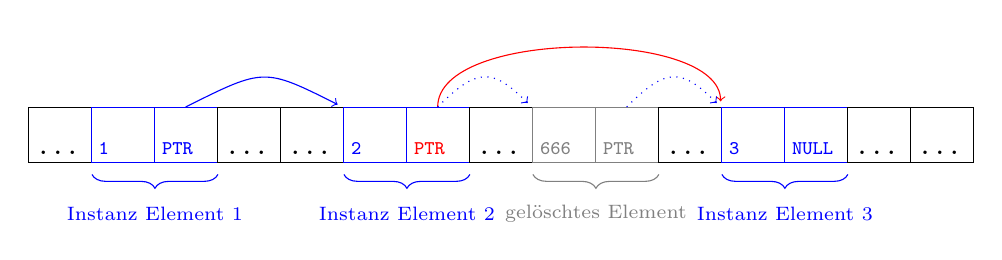
\begin{tikzpicture}
  [ 
    cell/.style={text width=6mm,
    text height=5mm, draw=black, inner sep=1mm},
    ld/.style={draw=blue,shorten >=2pt,->}
  ]

  \node (c01) at ( 0.0,0) [cell]         {\ttfamily \ldots};
  \node (c02) at ( 0.8,0) [cell, blue]   {\ttfamily \scriptsize 1};
  \node (c03) at ( 1.6,0) [cell, blue]   {\ttfamily \scriptsize PTR};
  \node (c04) at ( 2.4,0) [cell]         {\ttfamily \ldots};
  \node (c05) at ( 3.2,0) [cell]         {\ttfamily \ldots};
  \node (c06) at ( 4.0,0) [cell, blue]   {\ttfamily \scriptsize 2};
  \node (c07) at ( 4.8,0) [cell, blue]   {\ttfamily \scriptsize \textcolor{red}{PTR}};
  \node (c08) at ( 5.6,0) [cell]         {\ttfamily \ldots};
  \node (c09) at ( 6.4,0) [cell, gray]   {\ttfamily \scriptsize 666};
  \node (c10) at ( 7.2,0) [cell, gray]   {\ttfamily \scriptsize PTR};
  \node (c11) at ( 8.0,0) [cell]         {\ttfamily \ldots};
  \node (c12) at ( 8.8,0) [cell, blue]   {\ttfamily \scriptsize 3};
  \node (c13) at ( 9.6,0) [cell, blue]   {\ttfamily \scriptsize NULL};
  \node (c14) at (10.4,0) [cell]         {\ttfamily \ldots};
  \node (c15) at (11.2,0) [cell]         {\ttfamily \ldots};
  
  \draw [ld]         (c03.north) .. controls +(1.0,0.5) and +(-1.0, 0.5) .. (c06.north west);
  \draw [ld, red]    (c07.north) .. controls +(0.0,1.0) and +(-0.0, 1.0) .. (c12.north west);
  \draw [ld, dotted] (c07.north) .. controls +(0.5,0.5) and +(-0.5, 0.5) .. (c09.north west);
  \draw [ld, dotted] (c10.north) .. controls +(0.5,0.5) and +(-0.5, 0.5) .. (c12.north west);

  \draw [decorate, decoration={brace, amplitude=5pt, mirror}, xshift=-4pt, yshift=0pt, blue]
  		(0.55, -0.5) -- (2.15, -0.5) 
  		node [midway, yshift=-0.5cm]
		(I1) {\scriptsize Instanz Element 1};
  \draw [decorate, decoration={brace, amplitude=5pt, mirror}, xshift=-4pt, yshift=0pt, blue]
  		(3.75, -0.5) -- (5.35, -0.5) 
  		node [midway, yshift=-0.5cm]
		(I2) {\scriptsize Instanz Element 2};
  \draw [decorate, decoration={brace, amplitude=5pt, mirror}, xshift=-4pt, yshift=0pt, blue]
  		(8.55, -0.5) -- (10.15, -0.5) 
  		node [midway, yshift=-0.5cm]
		(I3) {\scriptsize Instanz Element 3};
  \draw [decorate, decoration={brace, amplitude=5pt, mirror}, xshift=-4pt, yshift=0pt, gray]
  		(6.15, -0.5) -- (7.75, -0.5) 
  		node [midway, yshift=-0.5cm]
		(I4) {\scriptsize gelöschtes Element};
\end{tikzpicture}
%
\begin{itemize}
\item Pointer des Vorgängers updaten
\item Speicher freigeben
\item Ähnliche Sonderfälle für Listenanfang und Listenende
\end{itemize}
\end{tcolorbox}
%
\end{frame}

% =========================================================================== %

\begin{frame}[fragile]
%
\begin{columns}[T]
\column{.5\linewidth}
\begin{Large}
{Problem Einstiegspunkt}
\vspace{6pt}
\end{Large}
%
\begin{itemize}
\item Einfügen und Löschen kann Einstiegspunkt verändern
\item Funktionen, die diese Aufgaben übernehmen müssen diese Information weiterleiten
\item Verwaltungsvariable muss sich ändern
\item Lösung: \emph{Zwei} Datentypen
	\begin{itemize}
	\item Listenelemente
	\item Verwaltungs-Variable
	\end{itemize}
\end{itemize}
%
\column{.5\linewidth}
\begin{codebox}[Datentypen für Listenelemente und Verwaltungsvariable einer Linked List]
\begin{minted}[linenos, fontsize=\scriptsize]{c}
typedef struct listElement_struct {
  void *                      data;
  struct listElement_struct * next;
} listElement_t;

typedef struct {
  listElement_t * first;
  int             size;
  
  int             memoryAutoManaged;
  void (*printElement)(void *);
} linkedList_t;
\end{minted}
\end{codebox}
\end{columns}
%
\end{frame}

% =========================================================================== %

\begin{frame}
%
\begin{center}
(Codebeispiel: Linked List)
\end{center}
%
\end{frame}

% =========================================================================== %

\begin{frame}{Anmerkungen zur Anwendung von Linked Lists}
%
\begin{itemize}
\item \emph{FIFO}: First in First Out
	\begin{itemize}
	\item Schnelles Einfügen/Löschen vom Anfang der Liste
	\item Mitte der Liste: \enquote{Durchhangeln} nötig
	\end{itemize}
\item Iteration über \emph{alle} Listenelemente: Leicht umsetzbar
\item Sortieren: Schwierig
\item[$\Rightarrow$] Auf spezielle Anwendungsfälle zugeschnitten
\item Andere Speicherstrukturen für andere Fälle
	\begin{itemize}
	\item Doubly Linked Lists (\enquote{LIFO}: Last In First Out)
	\item Binary Search Trees
	\item Red/Black-Trees
	\item \ldots
	\end{itemize}
\item Vorlesung \emph{Algorithmen und Datenstrukturen}
\end{itemize}
%
\end{frame}
\end{document}